\subsection{Experiments}
We experimented with shallow trees on various binary and multi-class datasets.
We report both assessment complexity and CPU time complexity for each dataset. Though \texttt{Adaptive-Pruning Boost} is a general Boosting algorithm, we experimented with the following class of algorithms (1) Boosting exact greedy-optimal decision trees and (2) Boosting approximate decision trees.

Each algorithm was run with either the state-of-the-art method (\texttt{Quick Boost}) or our decision tree training method (\texttt{Adaptive-Pruning Boost}), apart from the case of Figure~\ref{fig:wolb} that also uses the brute-force decision tree search method (\texttt{Classic AdaBoost}). The details of our datasets are in Table~\ref{datasets}. For datasets SATIMAGE, W4A, A6A, and RCV1 tree depth of three was used and for MNIST Digits tree depth of four was used (as in \citet{icml2013_appel13}). Train and test error results are provided as supplementary material.

\begin{table*}[ht]
\caption{The datasets used in our experiments.}
\label{datasets}
\vskip 0.15in
\begin{center}
\begin{small}
\begin{sc}
\begin{tabular}{llccc}
\toprule
Dataset & Source & Train / Test Size & Total Features & Classes\\
\midrule
a6a & \citet{Platt:1999:FTS:299094.299105} & 11220 / 21341 & 123 & 2 \\
MNIST Digits & \citet{726791} & 60000 / 10000 & 780 & 10 \\
rcv1 (Binary) & \citet{Lewis:2004:RNB:1005332.1005345} & 20242 / 677399 & 47236 & 2 \\
satimage & \citet{991427} & 4435 / 2000 & 36 & 6 \\
w4a & \citet{Platt:1999:FTS:299094.299105} & 7366 / 42383 & 300 & 2 \\
\bottomrule
\end{tabular}
\end{sc}
\end{small}
\end{center}
\vskip -0.1in
\end{table*}


\paragraph{Boosting Exact Greedy-Optimal Decision Trees.}
We used \texttt{AdaBoost} for exact decision tree training.
Figure~\ref{fig:wolb} shows the total number of example assessments used by AdaBoost when it uses three different decision trees building methods described above. In all of these experiments, our algorithm, \texttt{Adaptive-Pruning Boost}, not only consistently beats \texttt{Quick Boost} but it also almost matches the weight order lower bound. The \texttt{Classic AdaBoost} can be seen as the upper bound on the total number of example assessments.

Table~\ref{complexity-exact-results} shows that CPU time improvements correspond to example-assessments improvements for \texttt{Adaptive-Pruning Boost} for all our datasets, except for RCV1. This could be explained by Figure~\ref{fig:wolb} wherein \texttt{Quick Boost} is seen approaching the lower bound for this particular dataset. While \texttt{Adaptive-Pruning Boost} is closer to the lower bound, its example-assessments improvements are not enough to translate to CPU time improvements.

 \begin{figure*}[ht]
\centering
\begin{subfigure}{.31\linewidth}
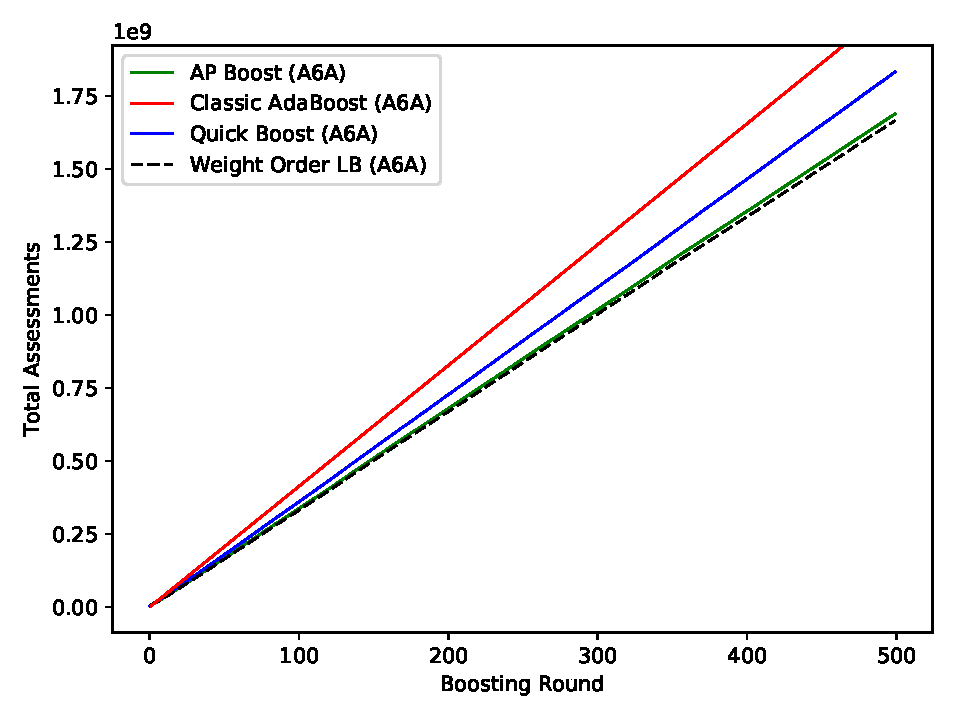
\includegraphics[width=\linewidth]{decisiontree/figures/result3_wolb_a6a}
\end{subfigure}
\begin{subfigure}{.31\linewidth}
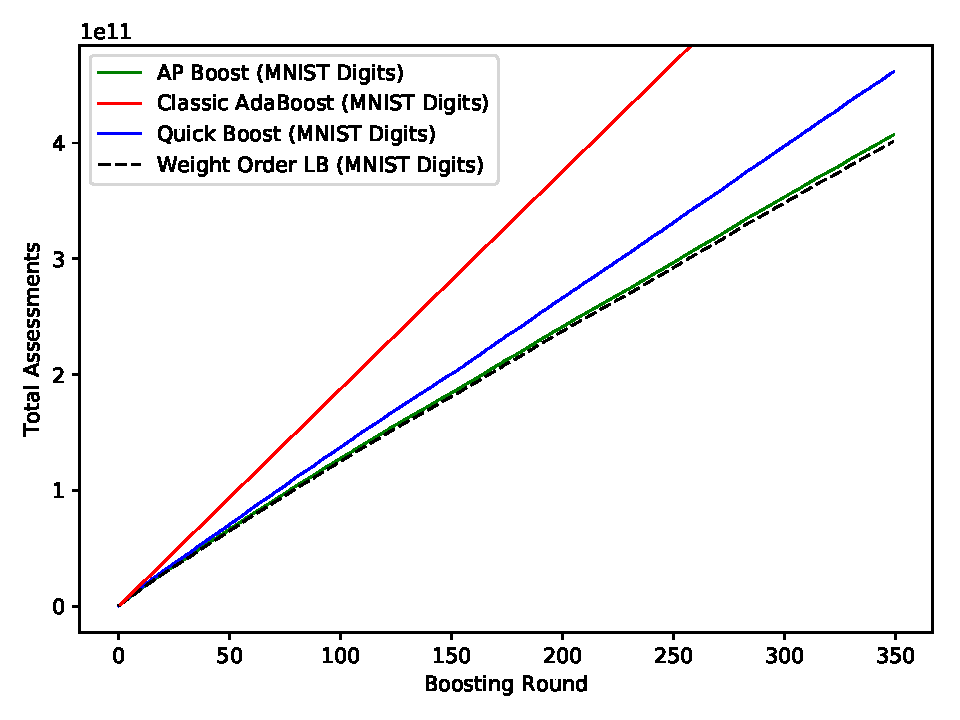
\includegraphics[width=\linewidth]{decisiontree/figures/result3_wolb_mnist}
\end{subfigure}
\begin{subfigure}{.31\linewidth}
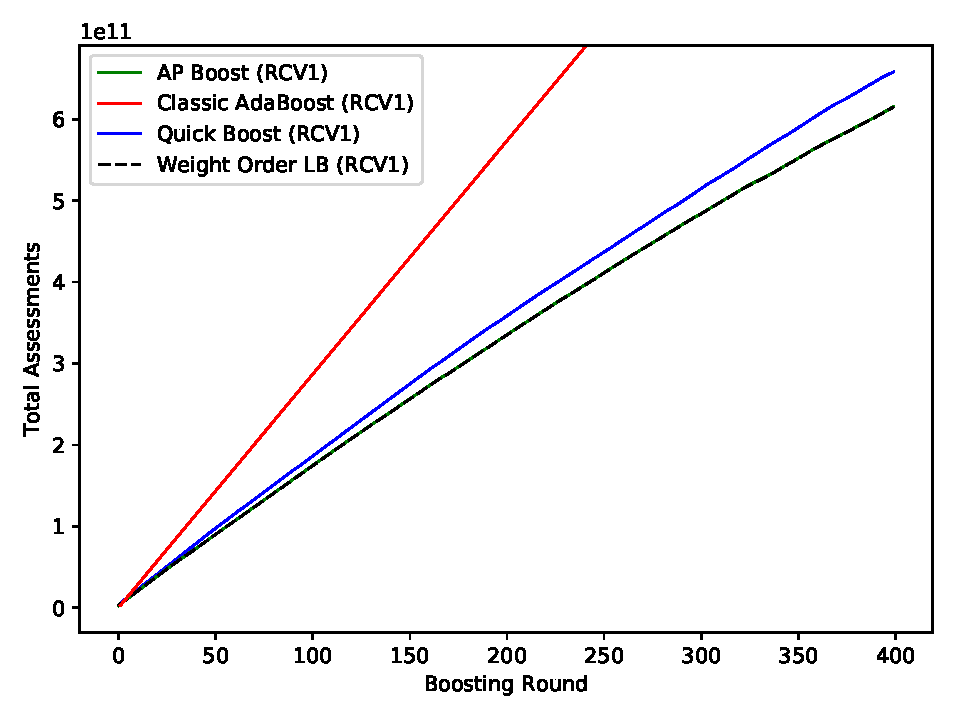
\includegraphics[width=\linewidth]{decisiontree/figures/result3_wolb_rcv1}
\end{subfigure}
\begin{subfigure}{.31\linewidth}
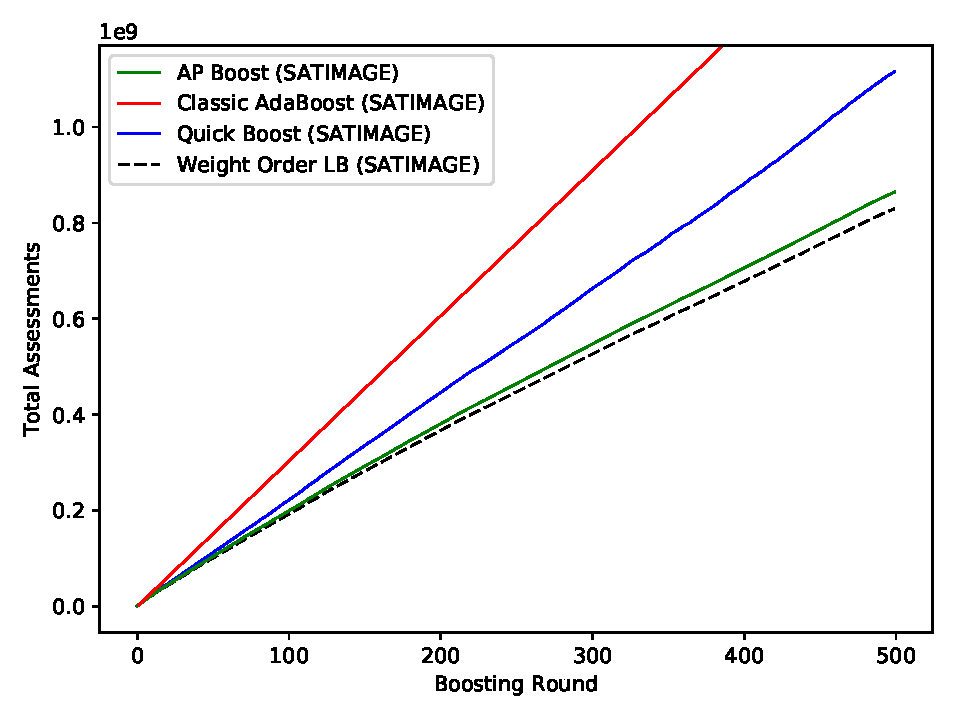
\includegraphics[width=\linewidth]{decisiontree/figures/result3_wolb_satimage}
\end{subfigure}
\begin{subfigure}{.31\linewidth}
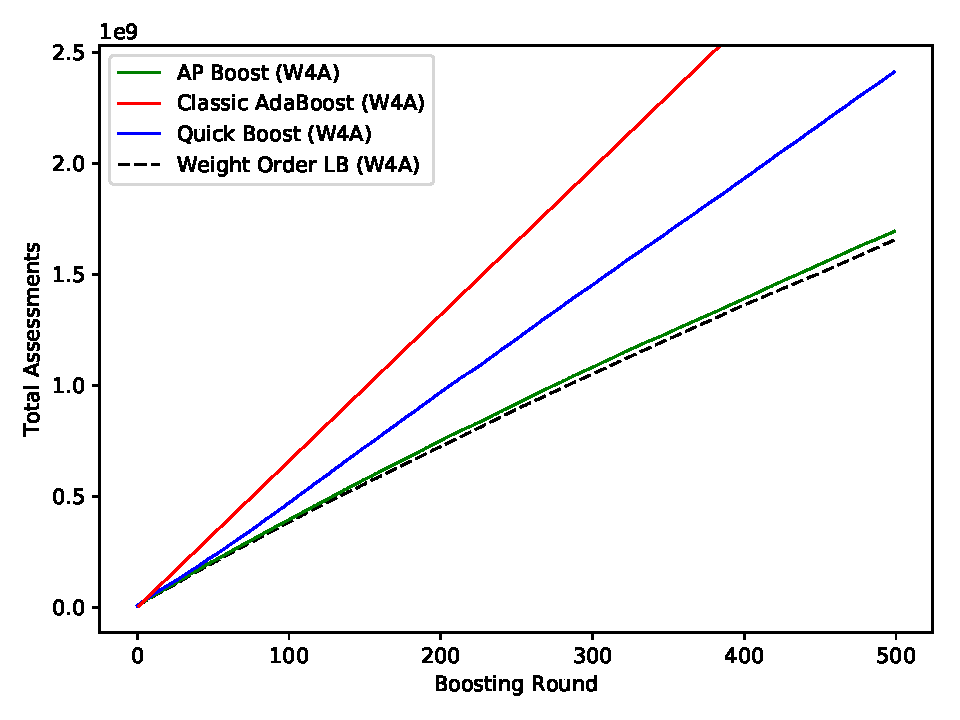
\includegraphics[width=\linewidth]{decisiontree/figures/result3_wolb_w4a}
\end{subfigure}
\caption{We report the total number of assessments at various boosting rounds used by the algorithms, as well as the weight order lower bound. In all of these experiments, our algorithm, \texttt{AP Boost}, not only consistently beats \texttt{Quick Boost} but it also almost matches the lower bound.}
\label{fig:wolb}
\end{figure*}

\begin{table*}[ht]
\caption{Computational Complexity for AdaBoost.
All results are for 500 rounds of boosting except MNIST (300 rounds) and RCV1 (400 rounds).}
\label{complexity-exact-results}	
\vskip 0.15in
\begin{center}
\begin{small}
\begin{sc}
\begin{tabular}{llccrccr}
\toprule
& & \multicolumn{3}{c}{CPU Time in Seconds} & \multicolumn{3}{c}{\# Example Assessments} \\
Dataset & Boosting & AP-B & QB & Improv. & AP-B & QB & Improv. \\
\midrule
a6a & AdaBoost & 4.49e+02 & 4.46e+02 & 5.3\% & 1.69e+09 & 1.83e+09 & 7.8\% \\
%
mnist & AdaBoost & 6.32e+05 & 6.60e+05 & 4.2\% & 3.52e+11 & 3.96e+11 & 11.1\% \\
%
rcv1 & AdaBoost & 1.58e+05 & 1.58e+05 & -0.5\% & 6.15e+11 & 6.58e+11 & 6.5\% \\
%
satimage & AdaBoost & 9.21e+02 & 1.19e+03 & 18.9\% & 8.64e+08 & 1.11e+09 & 22.5\% \\
%
w4a & AdaBoost & 3.03e+02 & 3.96e+02 & 27.1\% & 1.69e+09 & 2.41e+09 & 29.8\% \\
\midrule
Mean &  & &  & 11\% & & & 15.54\% \\
\bottomrule
\end{tabular}
\end{sc}
\end{small}
\end{center}
\vskip -0.1in
\end{table*}



\paragraph{Boosting Approximate Decision Trees.}
We used two approximate boosting algorithms.
We experimented with Boosting with Weight-Trimming 90\% and 99\% \citep{Friedman98additivelogistic}, wherein the weak hypothesis is trained only on 90\% or 99\% of the weights, and LazyBoost 90\% and 50\% \citep{Escudero:2001:ULW:2387364.2387381} wherein the weak hypothesis is trained only on 90\% or 50\% randomly selected features. Table~\ref{complexity-approx-results} shows that the CPU time improvements correspond to assessment improvements.

Note that approximate algorithms like XGBoost of \cite{Chen:2016:XST:2939672.2939785} are not competitors to \texttt{Adaptive-Pruning Boost} but rather potential ``clients'' because such algorithms train on a subset of the data. Therefore, they are not appropriate baselines to our method.
\begin{table*}[ht]
\caption{Computational Complexity for LazyBoost and Boosting with Weight Trimming.
All results are for 500 rounds of boosting except MNIST (300 rounds) and RCV1 (400 rounds).}
\label{complexity-approx-results}	
\vskip 0.15in
\begin{center}
\begin{small}
\begin{sc}
\begin{tabular}{llccrccr}
\toprule
& & \multicolumn{3}{c}{CPU Time in Seconds} & \multicolumn{3}{c}{\# Example Assessments} \\
Dataset & Boosting & AP-B & QB & Improv. & AP-B & QB & Improv. \\
\midrule
a6a & LazyBoost (0.5) & 1.86e+02 & 1.95e+02 & 4.8\% & 8.48e+08 & 9.22e+08 & 8.1\%  \\
mnist & LazyBoost (0.5) & 4.44e+05 & 4.57e+05 & 2.8\% & 1.84e+11 & 2.05e+11 & 10.3\% \\
rcv1 & LazyBoost (0.5) & 7.86e+04 & 7.54e+04 & -4.2\% & 3.18e+11 & 3.29e+11 & 3.4\% \\
satimage & LazyBoost (0.5) & 4.70e+02 & 5.48e+02 & 14.2\%  & 5.17e+08 & 6.11e+08 & 15.4\%  \\
w4a & LazyBoost (0.5) & 1.15e+02 & 1.58e+02 & 26.8\% & 8.61e+08 & 1.22e+09 & 29.3\% \\
\midrule
Mean &  & &  & 8.68\% & & & 13.18\% \\
\midrule
a6a & LazyBoost (0.9) & 3.28e+02 & 3.48e+02 & 5.6\%  & 1.51e+09 & 1.64e+09 & 7.7\%  \\
mnist & LazyBoost (0.9) & 7.63e+05 & 7.86e+05 & 2.9\% & 3.24e+11 & 3.62e+11 & 10.5\% \\
rcv1 & LazyBoost (0.9) & 1.38e+05 & 1.37e+05 & -1.0\% & 5.60e+11 & 5.93e+11 & 5.6\% \\
satimage & LazyBoost (0.9) & 7.37e+02 & 8.89e+02 & 17.1\%  & 8.05e+08 & 1.01e+09 & 20\%  \\
w4a & LazyBoost (0.9) & 2.04e+02 & 2.82e+02 & 27.7\% & 1.52e+09 & 2.19e+09 & 30.5\% \\
\midrule
Mean &  & &  & 10.54\% & & & 14.94\% \\
\midrule
a6a & Wt. Trim (0.9) & 2.69e+02 & 2.69e+02 & 0\%  & 1.23e+09 & 1.24e+09 & 1.4\%  \\
mnist & Wt. Trim (0.9) & 7.91e+05 & 9.49e+05 & 16.6\% & 4.61e+11 & 4.61e+11 & 0.0\% \\
rcv1 & Wt. Trim (0.9) & 8.87e+04 & 8.95e+04 & 0.9\%  & 3.65e+11 & 3.79e+11 & 3.6\% \\
satimage & Wt. Trim (0.9) & 9.87e+02 & 9.76e+02 & -1.2\%  & 1.26e+09 & 1.26e+09 & 0.1\%  \\
w4a & Wt. Trim (0.9) & 1.88e+02 & 1.96e+02 & 4.1\% & 1.40e+09 & 1.43e+09 & 2.5\% \\
\midrule
Mean &  & &  & 4.74\% & & & 1.52\% \\
\midrule
a6a & Wt. Trim (0.99) & 3.34e+02 & 3.38e+02 & 1.3\%  & 1.54e+09 & 1.58e+09 & 2.6\%  \\
mnist & Wt. Trim (0.99) & 7.46e+05 & 7.27e+05 & -2.6\% & 3.18e+11 & 3.33e+11 & 4.8\% \\
rcv1 & Wt. Trim (0.99) & 1.38e+05 & 1.37e+05 & -1.0\% & 5.61e+11 & 5.86e+11 & 4.4\% \\
satimage & Wt. Trim (0.99) & 6.49e+02 & 6.68e+02 & 2.9\%  & 7.01e+08 & 7.39e+08 & 5.1\%  \\
w4a & Wt. Trim (0.99) & 1.91e+02 & 2.03e+02 & 6.0\% & 1.44e+09 & 1.52e+09 & 5.3\% \\
\midrule
Mean &  & &  & 1.48\% & & & 4.7\% \\
\bottomrule
\end{tabular}
\end{sc}
\end{small}
\end{center}
\vskip -0.1in
\end{table*}



